\chapter{Background \& Related Work}
\label{chap:background}

\section{Case-based Recommendation}
Case-based recommendation traces its roots to case-based reasoning (\cite{aamodt94}).
Case-based reasoning is a problem solving methodology which makes use of a case-base (database) of past problem solving experiences as its source of knowledge. 
A typical case in a case-base consists of a \textit{problem specification} outlining the problem and a \textit{solution part} which describes the solution used to solve the corresponding problem.
Given a new problem at hand with a problem specification $P_s$, a case S is retrieved from the case-base whose problem specification is similar to $P_s$ and then the solution of S is adapted to come up with a solution for $P_s$(\cite{smyth2007}).
Case-based recommender systems are particularly suitable for generating recommendations when we are dealing with structured representations of items and there are similarity measures that can be defined across features in the particular domain. 
Many e-commerce web sites deal with products such as cameras, computers etc. which are usually represented in terms of their features in a structured way. 
Once suitable similarity measures are devised, case-based recommender systems are ready to be taken to the field.

Consider a user who specifies the following query to the system: "I need a camera having a resolution of 8 Megapixels, manufactured by Canon, with a price less than \$500".
A case-based recommender might retrieve all cameras that have 'Canon' as their manufacturer and are similar in terms of 'Price' and 'Resolution' as mentioned in user's query and display them as recommendations.
The similarity between a query $q$ and a camera $C$, is estimated according to weighted similarity model as:
\begin{equation}
\label{eq:sim}
Similarity(q, C) = \frac{\sum_{i=1}^{n}{w_i \times sim_i(q_i, C_i)}}{\sum_{i=1}^{n}w_i}
\end{equation}

According to equation \ref{eq:sim}, the similarity between a user query \textit{q} and camera \textit{C} is estimated 
as a weighted sum of individual similarities between the corresponding features of $q$ and $C$. 
\textit{n} is the total number of features.
The weights associated with each feature reflect the importance of that feature in the overall similarity calculation process. 
Individual feature level similarities are calculated according to the similarity function corresponding to the particular feature \textit{i} which is denoted by $sim_i$($q_i, C_i$).
These feature level similarities, also referred to as local similarities, are defined by domain experts at the time of system design.
The similarity between two price values $p_i$ and $p_j$ can be defined as follows:
\begin{equation}
\label{eq:localSim}
sim_{price}(p_i, p_j) = 1 - \frac{\lvert p_i - p_j \rvert}{max(P) - min(P)}
\end{equation}
$max(P)$ and $min(P)$ refer to the maximum and minimum values of $price$ feature of all products in the case-base respectively.
As we can see from Equation \ref{eq:localSim}, greater the difference between $p_i$ and $p_j$, lesser is the similarity between them.
Similarity measures for other numeric attributes of a product can be defined similar to Equation \ref{eq:localSim}.
Defining similarity measures for nominal attributes is challenging.
Specialized domain knowledge is required to estimate the similarities between the nominal feature (Eg:"manufacturer") values of two products.\\
Case-based recommenders can be classified into two categories - 'Single-shot systems' and 'conversational systems'.


\section{Single-shot Systems}
Single shot systems are reactive systems which respond to user's query by showing him a single list of $k$ items in a single interaction(\cite{smyth2007}).
An example of this system is the analog device recommender described in (\cite{wilke98}) 
The user expresses his initial preferences to the system in terms of attribute values.
The system recommends those op-amps which are most similar to his preferences. 

\begin{algorithm}[ht]
  \SetKwInOut{Input}{input}\SetKwInOut{Output}{output}
  \DontPrintSemicolon
  %\Input{$PM$, $IS$}

  $R \gets \{\}$\\
  $S \gets$ top $bk$ items similar to user query $q$\\
  \For{ $i\gets0$ \KwTo $k$ }{
    Sort $S$ by $Quality(q, P, R)$ for each case $P$ in S; \\
    $R \gets R + First(S)$;\\
    $S \gets S - First(S)$;\\
  }
  \Return $R$;\\
  \caption{BoundedGreedySelection}
  \label{algo:boundedGreedy}
\end{algorithm}
It is often desirable to have diverse products in the recommendation list returned by the single-shot systems.
Having diverse items in recommendation list helps the user to develop a better understanding of different parts of the product space.
This will also enable him to understand the trade-offs that exist between different product features.
There have been several attempts done to achieve diversity in recommendation lists.
\textit{Bounded Greedy Selection} procedure described in \cite{boundedGreedy} has been shown to be giving the best results in many recommendation scenarios. 
The general algorithm for this method is illustrated in Algorithm \ref{algo:boundedGreedy}.
In this method, the retrieval set $R$ is iteratively constructed till it contains $k$ (length of recommendation list) items.
The set $S$ containing top $bk$ items is considered in the beginning of recommendation procedure. 
%In the first step, the top item in $S$ is added to $R$ and removed from $S$.
In each iteration, quality scores of all items in set $S$ are computed using Equation \ref{eq:quality}.
Item that has the highest $quality$ score amongst all items in set $S$ is added to the set $R$ and removed from $S$. 
This step is repeated till the size of set $R$ is equal to $k$.
This continues till there are $k$ items in the set $R$.
%$quality$ score of a product w.r.t. the retrieval set $R$ is computed as follows:

\begin{equation}
\label{eq:quality}
Quality(q, P, R) = similarity(q, P) * RelDiversity(p, R)
\end{equation}

\begin{equation}
\label{eq:relDiversity}
RelDiversity(p, R)  = \frac{\sum_{i=1}^{\lvert R \rvert} (1.0 - similarity(p, r_i))} {\lvert R \rvert}
\end{equation}
In this way, diversity in introduced into the retrieved list without significantly compromising on the similarity to the query.
%Another method for improving diversity in a recommendation set was proposed in \cite{expertclerk}, where a set of where a set of 3 recommendations $p1$, $p2$ and $p3$ is presented to the user. 
%$p1$ is the most similar product to the user query, $p2$ is maximally dissimilar to $p1$ and $p3$ is the most dissimilar product to both $p1$ and $p2$. As we can see, the products $p2$ and $p3$ may not be very similar to the user query.
%
%The two methods of introducing diversity into the recommendation process discussed till now were based on the explicit characterization of diversity in being the opposite of similarity. 
%However, there are other approaches where diversity gets introduced as a by-product. 
%Compromise driven retrieval (CDR) (\cite{mcsherry03}) is a method where diversity gets introduced without its explicit characterization. 
%The central idea in CDR is to estimate the utility of a product for a user by taking into account the compromises the product might be making with respect to the user query along with the weighted similarity model.
%Compromises can be defined as the preferences of the user that the recommender system failed to satisfy.
%To identify if a particular feature has been compromised or not, dominance criteria like MIB (More is Better) and LIB (Less is Better) are used. 
%For example, let us consider $price$ of a camera to be LIB feature and assume that a user specifies ‘X’ as his preferred $price$. 
%If a product $P$ in the database has $price$ greater than ‘X’, then we say that $P$ involves a compromise across the $price$ feature with respect to the query.
%CDR operates according to the following utility estimation principle - a given product is more acceptable than another product if it is more similar to the user query and involves a subset of the compromises that the other item involves.



\section{Conversational Recommender Systems}
Single shot retrieval works well in situations where the user is quite sure of his preferences and can frame a query appropriately.
In situations when the user only has a vague idea of what he wants, he might not be able to frame his information need for the system to retrieve interesting products in a single iteration. 
%If the user is not satisfied with the products that he is shown, he has no other option but to revise his query and restart the recommendation process.

So in situations where user has a poor domain knowledge and is not clear about his preferences, it might be useful for the system to engage the user in an extended interaction taking his feedback in each cycle.
The system can use user`s feedback in each interaction cycle, revise its model of the user preferences and propose relevant products.
Conversational recommender systems are classified into two categories based on the type of feedback they solicit from the user.
The recommendation process of conversational systems is classified to be either as \textit{navigation by proposing} or \textit{navigation by asking} (\cite{shimazu01}).

\subsection{Navigation by Asking}
\begin{mdframed}
%
Inquirer:  Which movie should I rent for the weekend?\\
Advisor:   Which genre do you prefer? \\
Inquirer:  What types are there? \\
Advisor:   Action, Comedy, Drama, Mystery and Horror. \\
Inquirer:  I will probably take an action movie released in last three years. \\
Advisor:   What should be it's IMDb rating?\\
Inquirer:  It should be atleast 8.5 \\
Advisor: I'm sorry, there are no movies like that. \\
Inquirer:  I will then take a mystery movie then. \\
Advisor:  The movie 'Inception' is the best match for your criteria. \\
Inquirer:  I'll take that. \\
\end{mdframed}

In this mode of feedback, the user is asked questions about his preference for various feature values during interaction.
Thus, it proceeds in a question answer interaction where the user may question the response of the system and answer questions that are posed to him.
As we can see from the above example, this mode of getting user feedback requires a lot of cognitive effort on the part of the user.

It is generally accepted that the users are not particularly fond of long question answer sessions. 
Additionally, it is possible that the user might not be able to answer the question that the system might ask him. 
Oftentimes they will not know the answers to questions that demand a high-level of domain knowledge or they may reject questions that ask for sensitive or personal information.
%Finally, there are a lot of interfacing issues in implementing text based question answer system. 
%For example, expecting the users to answer specific questions in a text based format might not be appropriate in the context of recommendations over devices such as mobile phones (\cite{smyth2007}).





\subsection{Navigation by Proposing}
\begin{figure}
    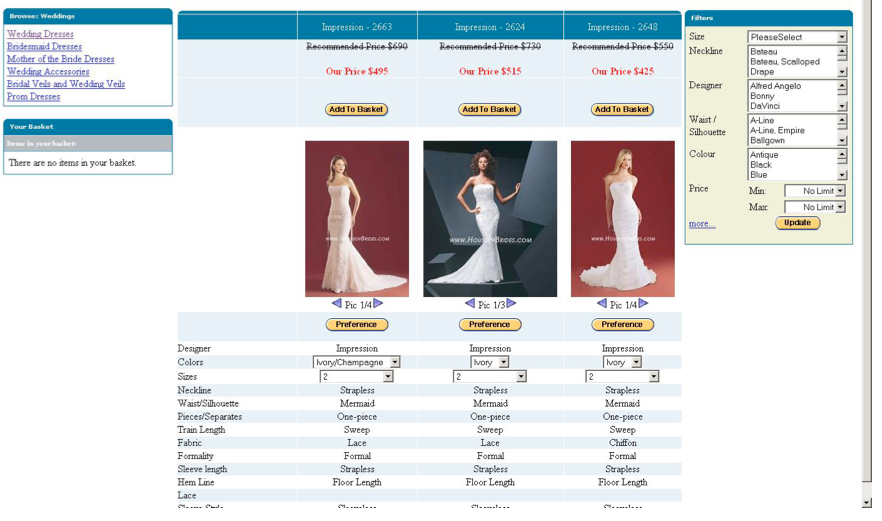
\includegraphics[width=1.0\textwidth]{figures-bharath/pbf.png}
  \caption{Recommender System that uses preference based feedback (\cite{smyth2007})}
  \centering
\label{fig:pbf2}
\end{figure}
%The limitations have of "Navigation by Asking" form of conversation as described above led to increased interest in other forms of user feedback.

The key feature of navigation by proposing is that the user is presented with one of more recommendation alternatives, rather than a question, during each recommendation cycle. 
The user is asked to offer feedback in relation to these alternatives.
There are three important kinds of feedback: Ratings-based feedback, Preference-based feedback and Critique-based feedback.\\
\\
\textbf{Ratings-based feedback:} In this kind of feedback, the recommender system provides a list of recommendations and  asks the user to provide an explicit rating for each item in the list.
One of the most famous systems that used this kind of feedback was the PTV system (\cite{smyth99tv}).
This system allows the user the grade the T.V. programs recommended to them into two categories - positive and negative. 
These ratings then are made part of the user profile which was used to generate further recommendations.\\
\\
\textbf{Preference-based feedback:} This is the simplest form of feedback which requires the user to indicate a preference for one recommendation over another. 
It is also particularly well suited to domains where users have very little domain knowledge.
Consider the example of the bridal dresses recommender system shown in Figure \ref{fig:pbf2}. 
The system shows 3 different items along with the feature values of each item in each cycle. 
The user can select one of the items as his preference.
The system takes user preference into account and generates 3 new recommendations in the next cycle.
Bridal wedding dresses is a good example of a domain where average shopper is likely to have a limited knowledge, in terms of the technical feature values of the items (\cite{smyth2007}).
However, most users will be able to select one dress as preference over the other.
Unfortunately, while this approach carries very little feedback overhead from a user’s perspective, it is ultimately limited in its ability to guide the recommendation process.
For example, a user might have chosen a particular item because he likes certain features of the item, but we can never be sure about which features compelled the user to select that item.
The system will have to then make an assumption that the user likes all of the features of the selected product and consequently, the quality of recommendations may not be very good.

\cite{comparisonbr} propose several query revision strategies to address the above problem.
The straightforward strategy(\textit{More Like This(MLT)}) simply adopts the preferred case as the new query and proceeds to retrieve the $k$ most similar cases to it for the next cycle.
This approach does not generate very efficient recommendations because it doesn't try to infer user's true preferences.
%There may be some features of the selected product that the user doesn't like.
An alternative approach(\textit{Partial More Like This(pMLT)}) transfers features from the preferred case only if these features are absent from all of the rejected cases, thus allowing the recommender to focus on those aspects of the preferred cases that are unique in the current cycle.
An another strategy(\textit{Weighted More Like This(wMLT)}) attempts to give weights to each of the features in the updated query according to how confident the recommender can be that these features are responsible for user's preference.
For example, in a Personal Computer(PC) recommender system, if the preferred PC has the manufacturer "Apple" and the other $k-1$ rejected PCs have different manufacturers, the system can give a high weight to 'manufacturer' attribute, since we can be confident that the particular user under consideration is genuinely interested in "Apple" computers.
On the other hand, if the preferred PC has a screen-size of 15 inches and all other $k-1$ rejected PCs also have the same screen-size, we can give a low weight to 'screen-size' attribute, since we cannot really infer whether the user is particularly interested in PCs with screen-size 15 inches.\\
\\
\begin{figure}
    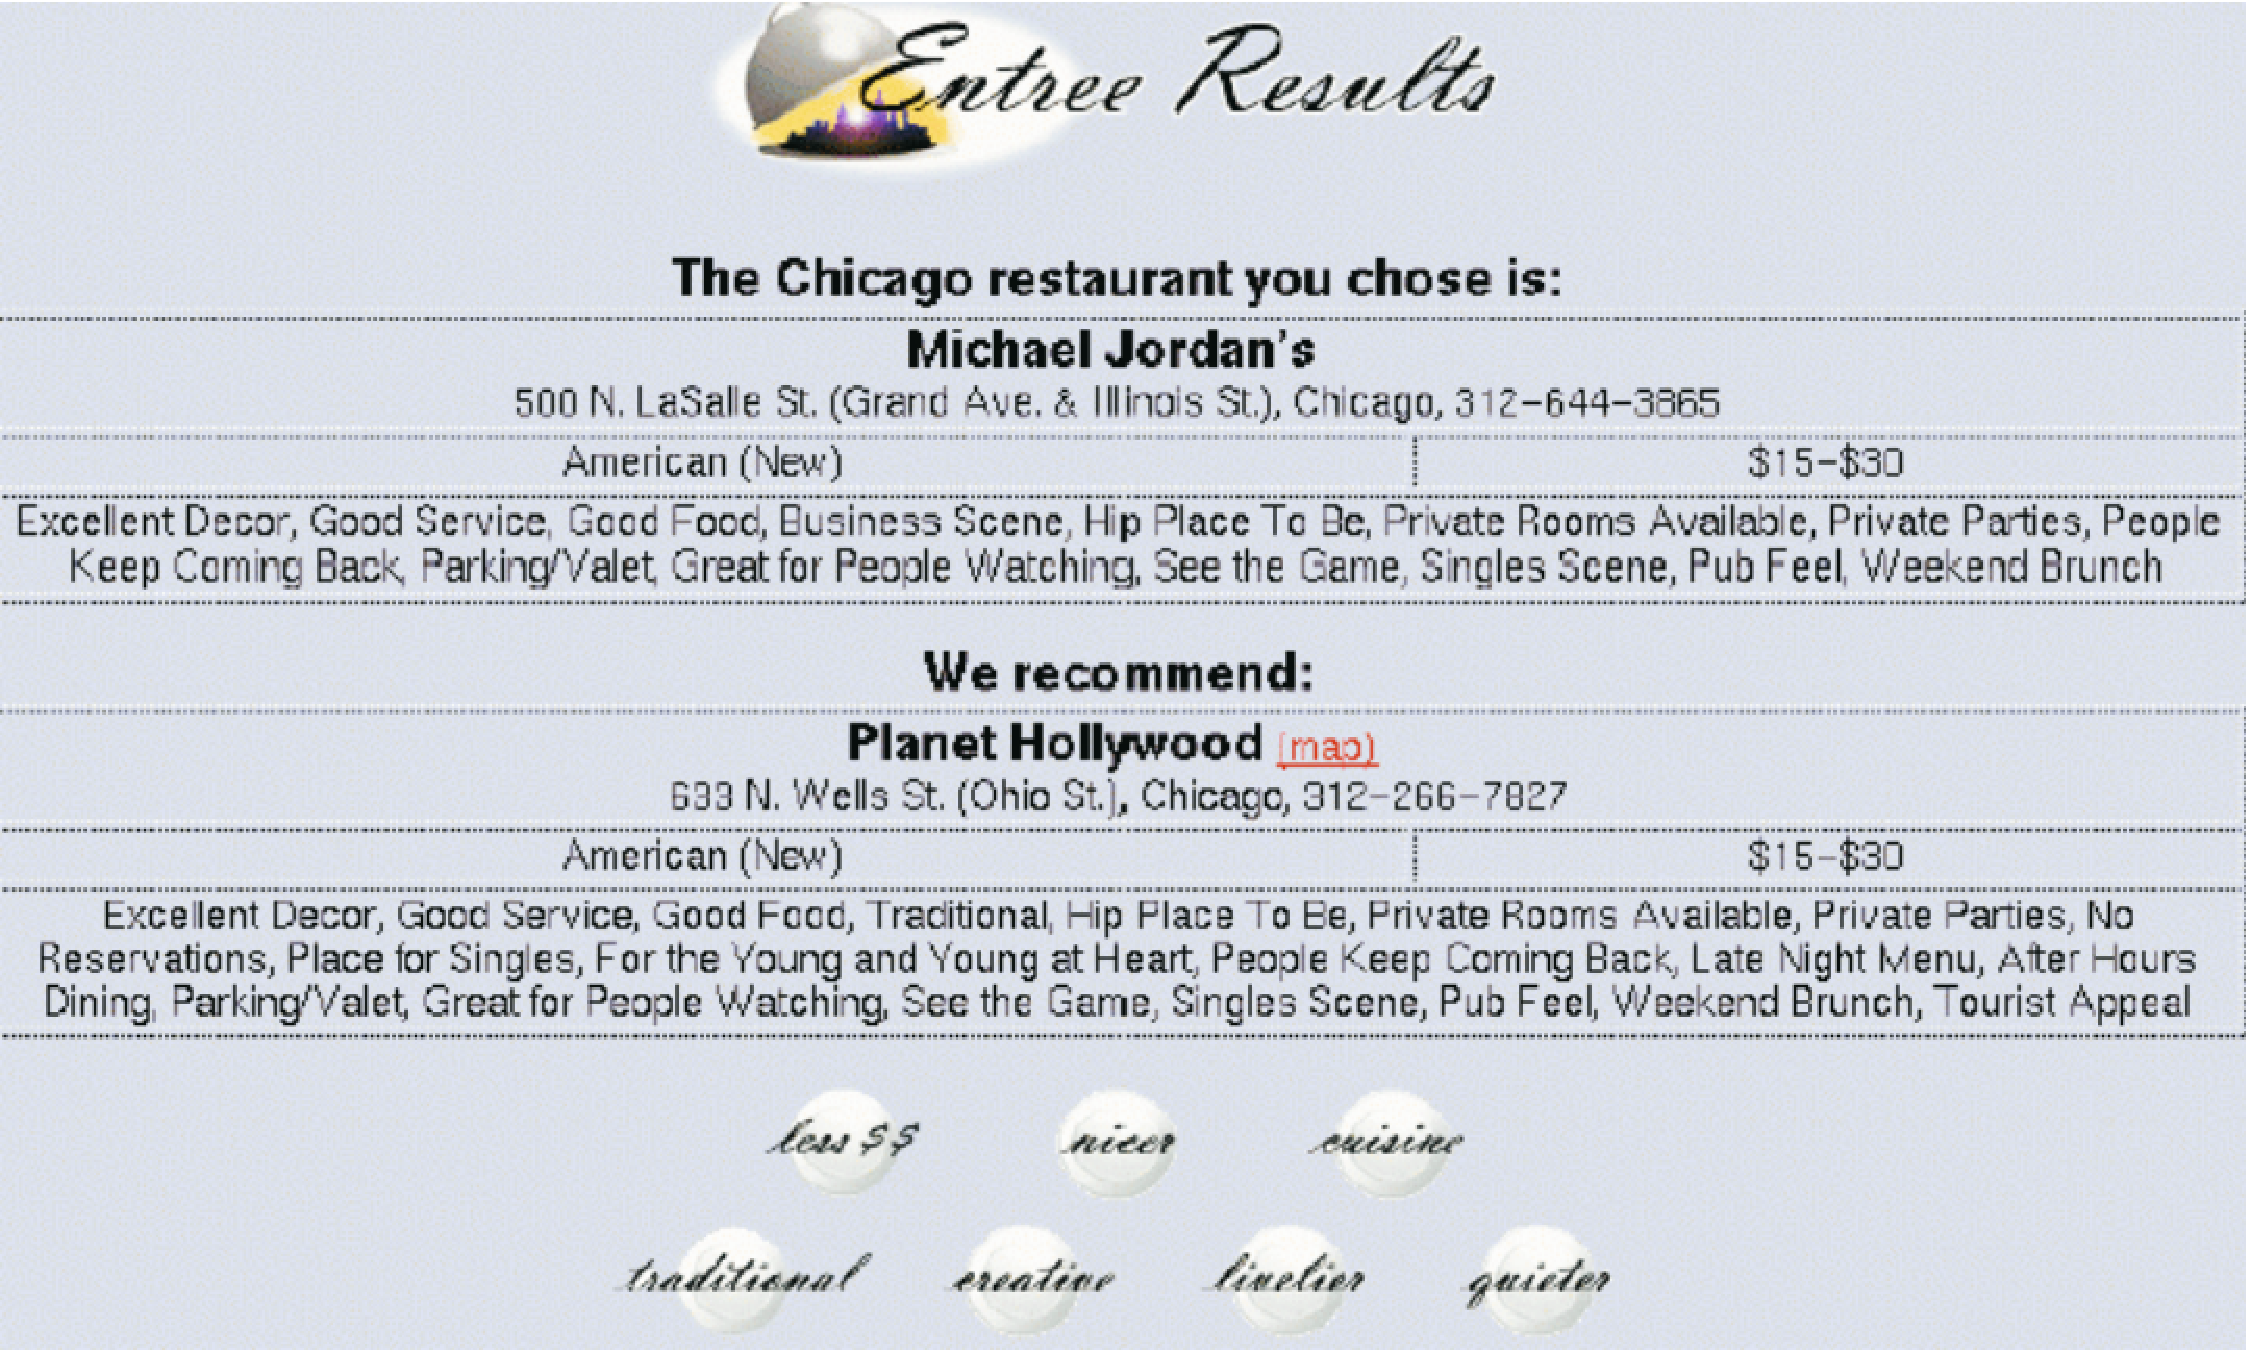
\includegraphics[width=1.0\textwidth]{figures-bharath/entree.pdf}
  \caption{Entree Restaurant Recommender System (\cite{entree})}
  \centering
\label{fig:entree}
\end{figure}
\textbf{Critique-based feedback:}
As already discussed in Section \ref{sec:critiquing}, critiquing based recommenders allow users to choose a product and provide directional preference(s) over one or more feature values of the product.
In many domains, we cannot assume that users will be able to express their preferences at the beginning of interaction.
 Most users will not have an idea of the trade-offs/compromises that exist between different features of a product.
 Instead, as users become more familiar with the domain and the product options available, their preferences often change and become more rigid.
Critique-based conversational recommenders offer support as users navigate the product space and help them to better understand their preference requirements. 
Instead of requiring users to specify their preferences from the outset, user preferences are built up over a series of \textit{recommendation cycles}. 
Feature critiques typically take the form of \textit{directional} or \textit{replacement} critiques. 
Through replacement critiques, user can request for the substitution of any value (i.e., aside from critiqued value) for a non-numeric feature (e.g., different manufacturer implies [! = manufacturer]).
Through directional critiques user can express a request to increase or decrease over one or more numeric attribute values (e.g., cheaper implies [$<$  price]). 

%The FindMe systems developed by \cite{burkeEarlierSystems} were the first to employ critiquing in web-based recommenders recognizing the need to focus on educating the user about the options space.
%The Entree recommender (Figure \ref{fig:entree}) suggests restaurants in Chicago and each recommendation allows the user to select from seven different critiques.
%When a user selects a critique such as \textit{cheaper}, Entree eliminates cases (restaurants) that do not satisfy the critique %from consideration in the next cycle, 
%and selects the case that is most similar to the current recommendation among the remaining cases; thus each critique acts as a filter over the cases.
%Originally, FindMe systems were developed as \textit{browsing assistants} that helped users browse through large information-spaces, such as restaurants (\textit{Entree}), automobiles (\textit{Car Navigator}), apartments (\textit{RentMe}), and movie rentals (\textit{Video Navigator}) using critiquing.
%Other examples of early critiquing based systems include: \textit{Apt Decision}(\cite{aptDecision}) and \textit{Automated Travel Assistant (ATA)} (\cite{ata}).
%More recent research has highlighted that there is a tension between the need for a user to explore the space of items to understand the options and desire for short recommendation dialog (\cite{mcginty11}).


Critiquing  provides users with a straight-forward mechanism to provide feedback, one that requires limited domain knowledge on the part of the user and it is easy to implement with even the simplest of interfaces.
Over the past decade, a variety of critique-based recommendation methodologies have been proposed.
Researchers have demonstrated the benefits of critiquing over other forms of feedback in conversational recommender systems.
The primary reason why critiquing has become so popular is that it strikes an acceptable balance between the effort that a user must expend when providing feedback and the information value it provides(\cite{mcginty11}).
In comparison to the standard value elicitation approach, critiquing is a very low-cost form of feedback (in terms of user effort) that provides a relatively unambiguous indication of the user's current requirement(as compared to preference-based feedback where the feedback can be ambiguous).
 Critiquing is also well-suited to even the most basic interfaces and to users with only a rudimentary understanding of certain recommendation domains.


%In Sections \ref{sec:evolutionBeg}  we discuss various challenges in critique-based recommendation that have been addressed by various researchers over the past decade.

Most early systems that implemented critiquing used \textit{unit critiques}.
Unit critiques operate only on a single feature in a recommendation cycle. 
This ultimately limits the ability of the recommender to narrow its focus which can result in unnecessarily long recommendation dialogues.
Furthermore, a user may not understand the feature trade-offs that exist within a particular domain.
An alternative strategy is to use \textit{compound critiques}, which operate on multiple features in a single recommendation cycle.
The application of compound critiques enables the user to take larger steps in the recommendation space and hence they can arrive very quickly towards their target product.
As seen in Section \ref{sec:critiquing}, \textit{static} critiques do not change as the recommendation session progresses. 
On the other hand, \textit{dynamic} critiques change in each interaction cycle.
In Sections \ref{sec:apriori} and \ref{sec:maut}, we discuss the two most popular approaches for generating dynamic critiques - Apriori Algorithm based approach  and Multi-Attribute Utility Theory (MAUT) based approach.




\section{Apriori Algorithm Based Generation of Dynamic Critiques}
\label{sec:apriori}
\begin{figure}
  \centering
    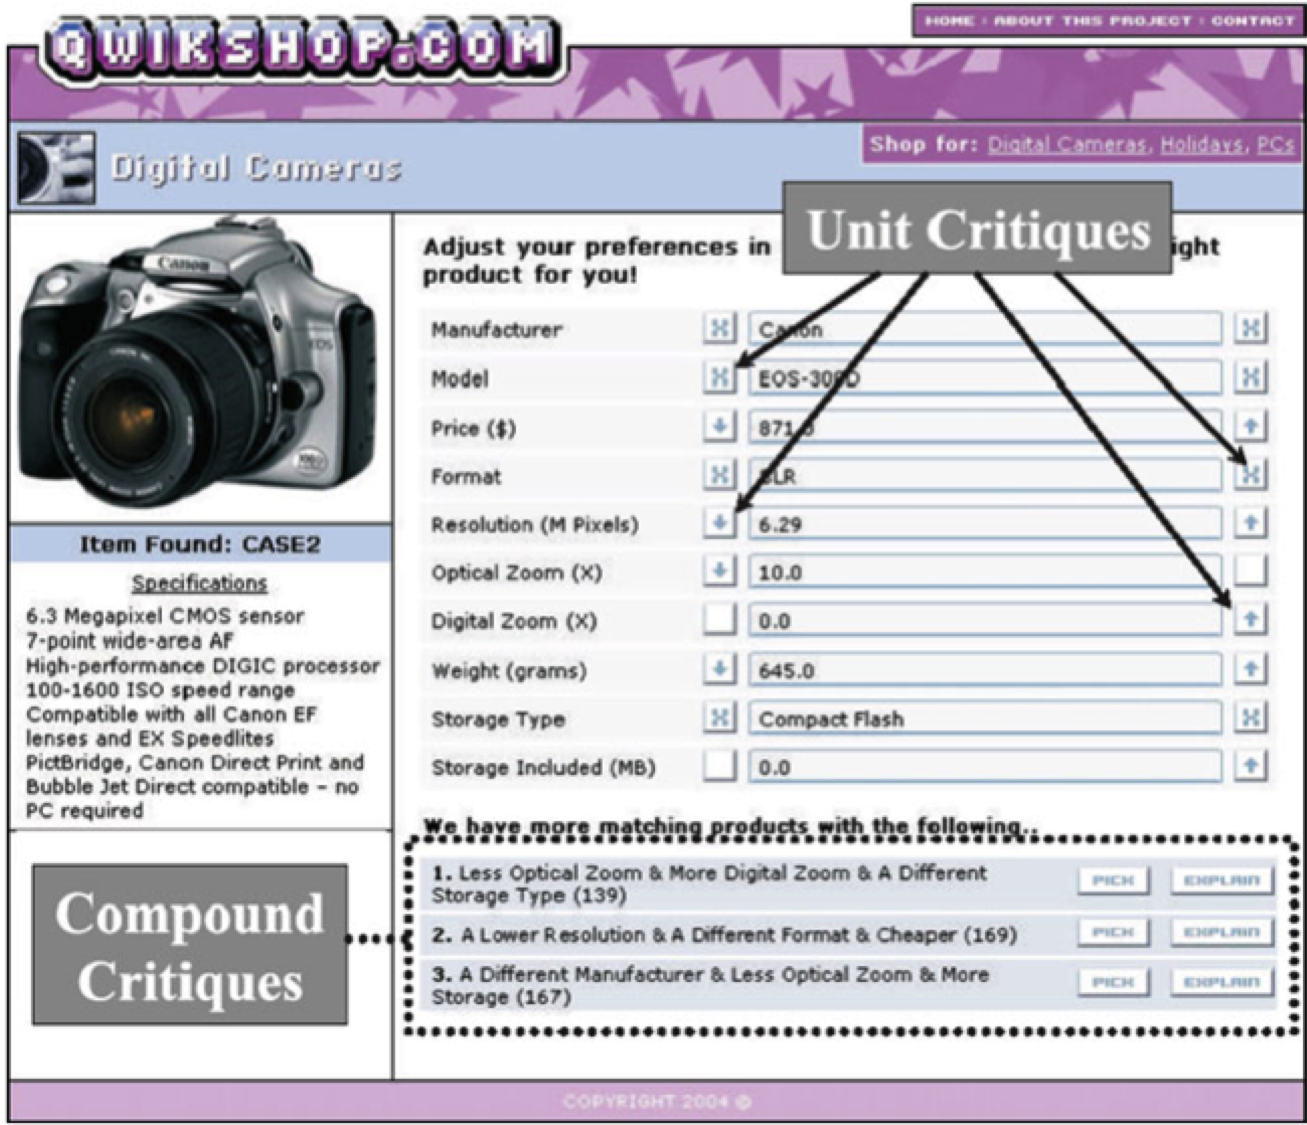
\includegraphics[width=0.8\textwidth]{figures-bharath/apriori.png}
  \caption{Screen-shot of digital camera recommender system that uses Apriori algorithm to generate compound critiques}
\label{fig:apriori}
\end{figure}
The screen-shot of a camera recommender system that uses Apriori algorithm to generate compound critiques is shown in Figure \ref{fig:apriori}.
 Each recommendation session will be commenced by an initial user query and this will result in the retrieval of the most similar case available for the first recommendation cycle.
In each recommendation cycle, only one product is displayed to the user.
The user can choose to either select this product and end the recommendation session, or critique the product.
In each cycle, the system presents unit critiques for each product feature  and a set of compound critiques(Figure \ref{fig:apriori}).
There are two steps involved in the generation of compound critiques: \textit{Generating Critique Patterns} and \textit{Mining Compound Critiques}.

\subsection{Generating Critique Patterns}
\label{sec:genCritique}
%\begin{figure}
%  \centering
%    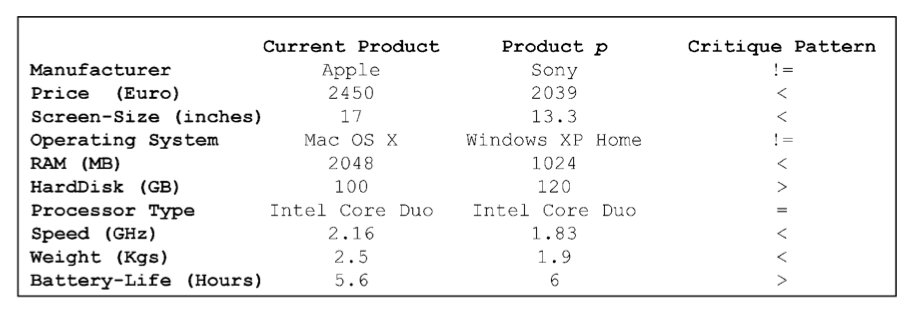
\includegraphics[width=1.0\textwidth]{figures-bharath/critiquePatterns.png}
%  \caption{Critique Pattern for the product p(\cite{reilly04})}
%\label{fig:critiquePatterns}
%\end{figure}

\begin{table}[h]
\caption{Generating Critique Patterns}
\centering
\renewcommand{\arraystretch}{1.2}
\label{tab:critiquePatterns}

\begin{tabular}{|l|l|l|l|}
\hline
& \textit{Current Product} & \textit{Product p} & \textit{Critique Pattern}\\
\hline
Manufacturer & Apple & Dell & $!=$\\
\hline
Processor Type & PowerPC G3 & Intel Core-i5 & $!=$\\
\hline
Processor Speed(MHz) & 1500 & 2000 & $>$ \\
\hline
Monitor (Inches) & 15  & 13 & $<$\\
\hline
Type & Laptop & Latop & $=$\\ 
\hline
RAM (MB) & 2048 & 4096 & $>$ \\
\hline
Drive Capacity(GB) & 500 & 320 & $<$ \\
\hline
Price (\$) & 1400 & 1000 & $<$\\
\hline
\end{tabular}
\end{table}

In any given interaction cycle, when the user selects a critique, remaining cases in the case base are filtered using that critique and the product that is most similar to previously recommended case is shown as the next recommendation.
We call this product as the \textit{current product}.
Each remaining case in the case-base is compared to the \textit{current product} to generate a so-called \textit{critique pattern}. 
Table \ref{tab:critiquePatterns} illustrates how critique pattern is generated.
As we can see in Table \ref{tab:critiquePatterns}, individual feature values of both the \textit{current product} and product $p$ are compared.
An attribute is \textit{numeric} if it can take numbers as its values.
An attribute is \textit{non-numeric} or \textit{nominal} if it can take only a fixed number of possible values.
'$<$', '$>$' and '$=$' are the possible values for numeric attributes in the critique pattern.
'$!=$' and '$=$' are the possible values for non-numeric attributes (Eg: manufacturer).
The critique pattern includes the critique [Price \textless] because the comparison product $p$ is less expensive compared to the \textit{current product}.
These patterns serve as the source of compound critiques.


\subsection{Mining Compound Critiques}
In this step, we would like to recognize useful recurring subsets of critiques within the large collection of critique patterns.
For example, if we find 40\% of the remaining cases have a lower price and lower screen size; and if user is actually looking for PCs that are cheaper and have smaller screen size, the application of this critique will immediately filter out 60\% of the remaining cases enabling the user to arrive at his product very quickly.
Apriori Algorithm (\cite{aprioriAlgo}) is used to generate recurring item subsets as association rules in the form of $A \rightarrow B$.
Apriori measures the importance of a rule in terms of \textit{support} and \textit{confidence}.
The support of a rule $A \rightarrow B$ is the percentage of patterns for which the rule is correct.
Confidence is the ratio of the number of patterns that contain both $A$ and $B$ and the total number of patterns that contain $A$.
For example, the rule [Monitor $<$] $\rightarrow$ [Price $<$] has support 0.6 if there are 100 critique patterns but only 60 of them contain both [Monitor $<$] and [Price $<$]. 
The confidence of the rule would be 0.75 if exactly 80 critique patterns contain [Monitor $<$].
During any given cycle, there will be a large number of association rules/ compound critiques mined by the Apriori algorithm.
It is not feasible to present all of the compound critiques to the user.
\cite{mccarthy2004dynamic} have experimentally observed that when compound critiques with low support values are presented in each cycle, the average number of interaction cycles in a recommendation session is minimum.
A compound critique with a low support value means that it is present in a small proportion of critique patterns and thus it is only applicable to a few remaining cases. 
If applied, the critique will therefore eliminate many cases from consideration.
Thus we can intuitively understand why application of compound critiques with low support reduces the number of interaction cycles.



\section{Multi Attribute Utility Theory (MAUT) based Generation of Dynamic Critiques}
\label{sec:maut}
Apriori algorithm based generation of compound critiques described in Section \ref{sec:apriori} was one of the first proposed approaches to dynamic critiquing.
It was proven to offer significant benefits in terms of reduction of number of interaction cycles compared to other approaches that use unit critiques (\cite{aprioriUserStudy}).
However, there is a serious limitation to the above approach - it does not take user's preferences into account while generating compound critiques.
There is no guarantee that the compound critiques generated by this methodology will be relevant to the user, since only product domain knowledge is utilized in generation of compound critiques.
\cite{mautPaper} propose an alternative methodology that relies on user preference knowledge.
They use Multi Attribute Utility Theory (MAUT) for dynamically generating compound critiques.
\begin{figure}
  \centering
    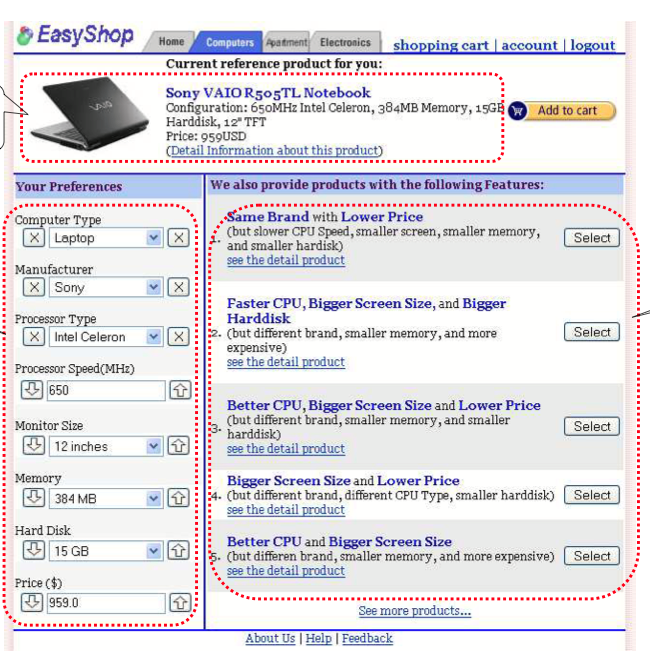
\includegraphics[width=0.8\textwidth]{figures-bharath/maut.png}
  \caption{Screen-shot of user interface of the recommender system that uses MAUT to generate compound critiques(\cite{mautPaper}}
\label{fig:maut}
\end{figure}

%\begin{figure}
%  \centering
%    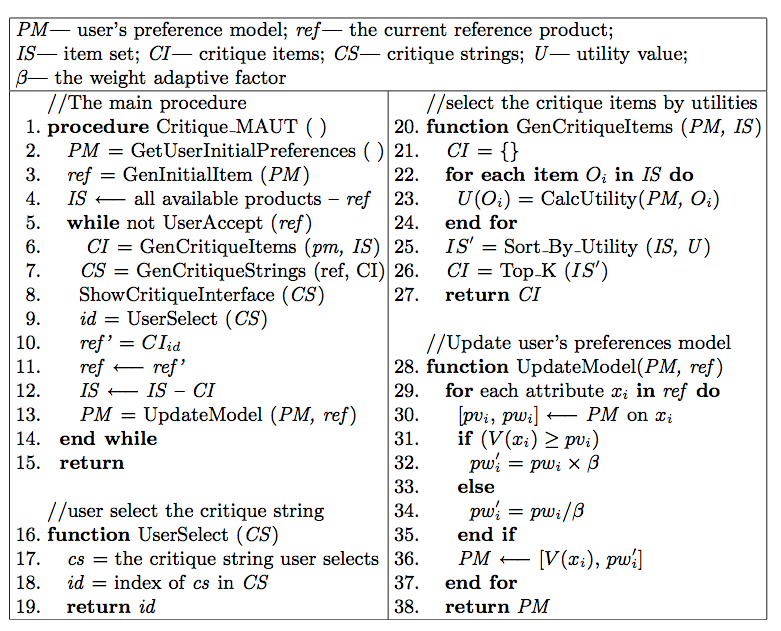
\includegraphics[width=0.9\textwidth]{figures-bharath/paperAlgo.png}
%  \caption{Algorithm for critiquing based on MAUT (\cite{mautPaper}}
%\label{fig:paperAlgo}
%\end{figure}

\begin{algorithm}[ht]
  \SetKwInOut{Input}{input}\SetKwInOut{Output}{output}
  \DontPrintSemicolon
    $PM$ = userQuery();\\
    $ref$ = generateFirstItem();\\
    $CB$ = $CB$- $ref$;\\
    \While {user does not accept $ref$}{
        $topK$ = GenCritiqueItems($PM$, $CB$);\\
        $CS$ = convertToStrings($ref$, $topK$);\\
        showInterface(CS);\\
        $index$ = userSelectedString(CS);\\
        $ref$ = $topK[index]$;\\
        $CB$ = $CB$ - $topK$;\\
        $PM$ = UpdateModel($PM$, $ref$);\\
    }
\caption{Critique\_MAUT()}
\label{algo:paperAlgo}
\end{algorithm}

\begin{algorithm}[ht]
  \SetKwInOut{Input}{input}\SetKwInOut{Output}{output}
  \DontPrintSemicolon
    \For{each item $p$ in CB} {
        $U(p)$ = CalcUtility($PM$, $p$);\\
    }
    $CB'$ = SortByUtility($CB$, $U$);\\
    \Return topK($CB'$);
\caption{GenCritiqueItems($PM$, $CB$)}
\label{algo:genItems}
\end{algorithm}

\begin{algorithm}[ht]
  \SetKwInOut{Input}{input}\SetKwInOut{Output}{output}
  \DontPrintSemicolon
  %\Input{$PM$, $IS$}

  $retVal \gets 0$;\\
  \For{ each attribute $x_i$ in $u$ }{
      retVal += $pw_i \times V(x_i)$
  }
  \Return retVal
  \caption{CalcUtility(PM, u)}
  \label{algo:utility}
\end{algorithm}


MAUT is a well-known  and powerful method in decision theory for ranking a list of multi-attribute products according to their utilities.
\cite{mautPaper} use a very simple additive form to calculate the utility of a product $O = \langle x_1,\hdots,x_n\rangle$ as described below:
\begin{equation}
\label{eq:utility}
U(\langle x_1,\hdots,x_n \rangle) = \sum_{i=1}^n w_iV_i(x_i)
\end{equation}
%
In Equation \ref{eq:utility}, $n$ is the number of attributes that each of the products has, $w_i$ is the weight/importance associated with the attribute $i$. 
$V_i$ is the value function associated with the attribute $i$ and it is given by experts during design time.
The algorithm for MAUT based compound critiquing is illustrated in Algorithm \ref{algo:paperAlgo}.
The functions \textit{GenCritiqueItems} and \textit{CalcUtility} have also been illustrated in Algorithms \ref{algo:genItems} and \ref{algo:utility} respectively.
The authors use a preference model which contains the weights and preferred values of product attributes to represent user's preferences.
The weights of all numeric attributes are initialized to $1/n$.
At the beginning of the interaction process, user gives some initial preferences to the system (Eg: \textit{HardDisk} = 500GB, \textit{Price} $<$ \$400 etc.).
In each interaction cycle, Critique\_MAUT approach will determine the top $K$ (=5) products with maximum utilities.
Each of the $K$ products is converted into a critique string by comparing it with the current reference product.
Determining critique string from a product is similar to generating critique patterns described in Section \ref{sec:genCritique}

In a given interaction cycle, when the user selects one of the critique strings, the product corresponding to the selected string is made as the reference product in the next cycle and user's preference model is updated based on this selection.
For each attribute, the attribute value of the new reference product is assigned as the preference value.
For LIB attributes(Eg: Price), if the new preference value is lesser than the old preference value, we want to favor lesser priced products in the next cycle and hence the weight of attribute 'Price' is multiplied by a factor $\beta$.
On the other hand, if the new preference value is greater than the old preference value, the weight of 'Price' attribute is divided by $\beta$.
For MIB attributes(Eg: HardDisk capacity), if the new preference value is higher than the old preference value, weight of the attribute is multiplied by $\beta$. Else, it is divided by $\beta$.
The authors set $\beta = 2.0$ in practice.
All the top $K$ products are removed from the case-base before the beginning of the next cycle.
Based on the new reference product and new preference model, the system recommends another set of critiques in the next cycle.
This process continues till the user find his target product and terminates the recommendation session.
Figure \ref{fig:maut} shows a screen-shot of PC recommender system developed based on the above approach.

\subsection{Value functions of numeric attributes}
In \cite{mautPaper}, the value functions of numeric attributes that were used in their implementation are not mentioned.
In our implementation, we first classify numeric attributes into two categories - LIB (Less is Better) and MIB (More is Better).
For the Camera dataset, the attribute \textit{Price} is classified into LIB, since given two cameras which have all other features the same, users would prefer the camera which has lower \textit{Price}.
Similarly, the attribute \textit{Weight} is classified into LIB.
The attributes \textit{Optical Zoom}, \textit{Digital Zoom}, \textit{Storage Included} and \textit{Resolution} are classified as MIB attributes.
The value function for LIB attributes and MIB attributes is given in Equations \ref{eq:valueLIB} and \ref{eq:valueMIB} respectively. $i$ refers to the attribute, $x_i$ is the value of product's $i^{th}$ attribute, $max_i$ and $min_i$ are the maximum and minimum values of the attribute among all the products in the case base.

\begin{equation}
\label{eq:valueLIB}
V_i(x_i) =  \frac{max_i - x_i}{max_i - min_i}
\end{equation}

\begin{equation}
\label{eq:valueMIB}
V_i(x_i) =  \frac{x_i-min_i}{max_i - min_i}
\end{equation}


\subsection{Updating value functions of nominal attributes}
\label{sec:valueFunc}
%As discussed earlier, in \cite{mautPaper}, the value functions that were used in the implementation are not mentioned.
For nominal attributes (Eg:manufacturer), we assume that all 'manufacturers' have equal value in the beginning of recommendation session.
In that case, updating only the weights of nominal attributes in each cycle will not affect rankings because the $w_i*V_i(x_i)$ term for all cases in case-base will be the same.
%Instead of updating the weights of nominal attributes in each iteration, we update their value functions.
Therefore, we update the value functions of nominal attributes instead of their weights.
The weights of all nominal attributes at the beginning of a recommendation session are initialized to $1$.
Let $v_1, v_2, v_3,\hdots v_k$ be $k$ possible values that a nominal attribute $N$(say manufacturer) can assume.
Value associated with each of $v_1, v_2, v_3,\hdots, v_k$ is initialized to $1/k$ at the beginning of interaction.
In the first cycle, if selected product's manufacturer is $v_1$, value associated with $v_1$ is changed to $(1+\gamma)/(k+\gamma)$; and the value associated with $v_2, v_3, \hdots, v_k$ will be $1/(1+\gamma)$ in the next cycle.
For example, if there are 4 different possible manufacturers for a PC -Apple, Toshiba, Compaq and HP, the values associated with each of the manufacturers at the beginning of the recommendation session will be 1/4.
Let $\gamma$ = 1.
If a HP manufactured PC is selected by the user in the first cycle, the value associated with HP after the first cycle will be 2/5 and the values associated with Apple, Toshiba and Compaq are 1/5.
In general, in cycle $t$,  each of $v_1, v_2, v_3,\hdots, v_k$ is multiplied by $(1 + t\gamma)$; if $v_p$ is the value of attribute $N$ in the selected product, then value associated with $v_p$ is increased by $\gamma$ and all the value functions associated with attribute $N$ are then normalized (so they all sum up to 1)  by dividing them all by $(1+ (t+1)\gamma)$.
%We fix $\gamma = 0.5$ in the implementation of the original MAUT based recommendation.


%\subsection{Function to calculate utility of products}
%\label{sec:utility}
%The function $CalcUtility(PM, u)$ is as follows:
%





\section{Offline Experiments}
\label{sec:offline}
%\begin{figure}
%\centering
%\begin{minipage}{.45\textwidth}
%  \centering
%  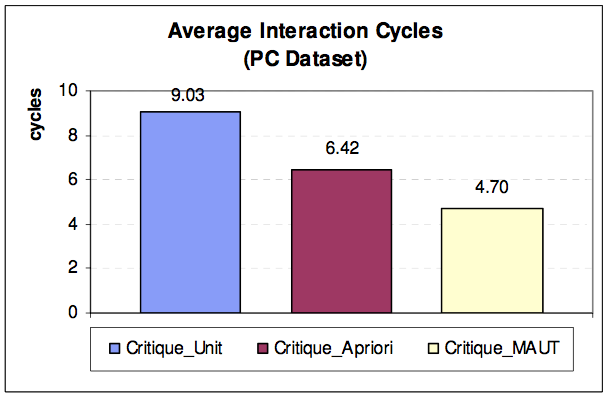
\includegraphics[width=1\linewidth]{figures-bharath/pc_results.png}
%  \captionof{figure}{Average interaction cycles for PC Dataset(\cite{mautPaper})}
%  \label{fig:pc_results}
%\end{minipage}%
%\;\;\;\;\;\;
%\begin{minipage}{.45\textwidth}
%  \centering
%  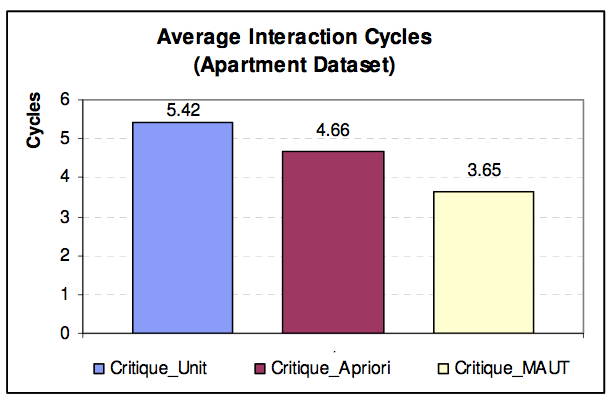
\includegraphics[width=1\linewidth]{figures-bharath/apartment_results.png}
%  \captionof{figure}{Average interaction cycles for Apartment dataset(\cite{mautPaper})}
%  \label{fig:apartment_results}
%\end{minipage}
%\end{figure}

\begin{table}
\caption{Average number of interaction cycles for PC and Apartment Datasets(\cite{mautPaper})}
\centering
\renewcommand{\arraystretch}{1.2}
\label{tab:paperResults}

\begin{tabular}{|p{5cm}|p{3cm}|p{3cm}|}
\hline
& PC & Apartment \\
\hline
Critique\_Unit & 9.03 & 5.42 \\
\hline
Critique\_Apriori & 6.42  & 4.66\\
\hline
Critique\_MAUT & \textbf{4.70} & \textbf{3.65}\\
\hline

\end{tabular}
\end{table}


%\begin{figure}[tbh]
%  \centering
%  \subfloat[PC Dataset]{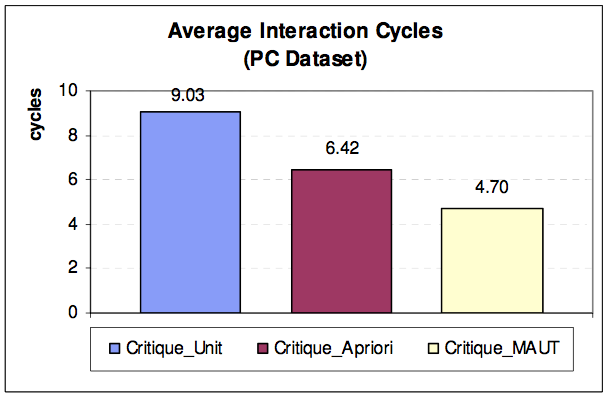
\includegraphics[width=.45\textwidth]{figures-bharath/pc_results}\label{fig:pc_results}} \hspace{.05\textwidth}
%  \subfloat[Apartment Dataset]{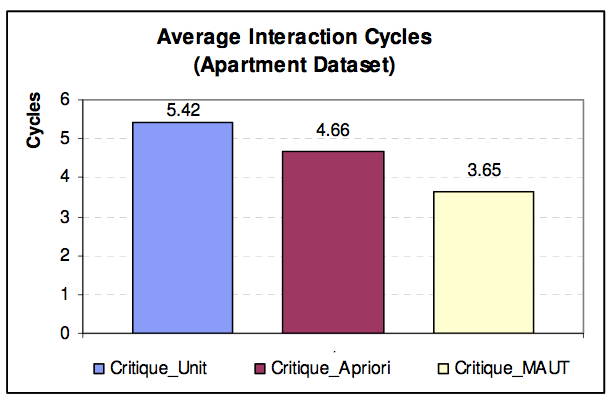
\includegraphics[width=.45\textwidth]{figures-bharath/apartment_results}\label{fig:apartment_results}}
%  \caption{Average interaction cycles for PC and Apartment datasets}
%\end{figure}
%Ideally, we would like to conduct live user studies to test the effectiveness of system generated compound critiques, but live user studies are very expensive to conduct.
%Instead we conduct offline evaluations to test the effectiveness of a recommendation algorithm.
\cite{mautPaper} conducted a set of simulation experiments to compare the performance of the basic unit critiquing approach (Critique\_Unit), the Apriori algorithm (Critique\_Apriori) and MAUT based generation of compound critiques (Critique\_MAUT).
The evaluation has been done based using a modified version of \textit{leave-one-out} method, a well-known offline evaluation mechanism for knowledge based systems.

For each experiment, the number of preferences($N$) in user's initial query are fixed at a constant (Eg: 1,3,5) at the beginning of evaluation.
A product $C$ is selected from the dataset and $N$ randomly selected attributes of the product are used to formulate user's initial query.
Product $C$ is the target product for the recommender system.
In each cycle of Critique\_MAUT, the simulated user is presented with five compound critiques that correspond to the five highest utility products.
The simulator calculates the compatibility of each compound critique with respect to the target product.
For example, considering PC domain, if a compound critique string is "Lesser Price, Larger screen size and Lower Hard-disk capacity", and the target product has "Higher Price, Larger screen size and Higher hard-disk capacity" with respect to current reference product, the compatibility of the given compound critique with the target product is 2/3 (2 out of 3 attributes have same direction as that of the target).
The simulated user selects the compound critique that is most compatible with the target product.
In case of a tie, he selects the critique whose corresponding product has a higher utility.
Based on the critique that the simulated user selects, the system changes the reference product and provides another set of critiques in the next cycle.
This interaction continues till the target product $C$ appears in the top five products.
Each product in the dataset is appointed as the target product 10 times and the average number of interaction cycles for all the experiments is calculated.

Two different datasets were used in the experiments: apartment data-set containing 50 apartments with 6 attributes: \textit{type, price, size, bathroom, kitchen,} and \textit{distance}.
The PC dataset contains contains 120 PCs with 8 different attributes. 
Table \ref{tab:paperResults} shows the average interaction cycles for PC, apartment datasets for different approaches.
Critique\_MAUT approach reduces the number of interaction cycles by 20\% compared to Critique\_Apriori approach.


\section{Live User Studies}
\label{sec:liveUser}
%write a paragraph of the results of the paper that conducted the live-user studies.

%\begin{figure}
%\centering
%\begin{minipage}{.45\textwidth}
%  \centering
%  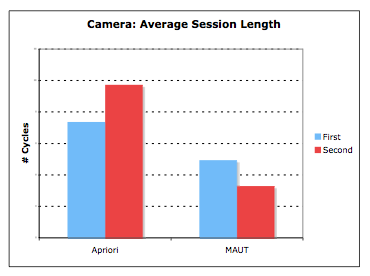
\includegraphics[width=1\linewidth]{figures-bharath/camera_liveUser.png}
%  \caption{Avg. session lengths on camera dataset (\cite{liveUserStudy}}
%  \label{fig:camera_liveUser}
%\end{minipage}%
%\;\;\;\;\;\;
%\begin{minipage}{.45\textwidth}
%  \centering
%  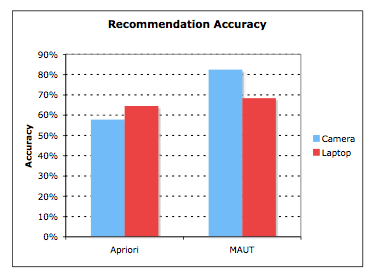
\includegraphics[width=1\linewidth]{figures-bharath/accuracy_liveUser.png}
%  \caption{Avg recommendation accuracy (\cite{liveUserStudy})}
%  \label{fig:accuracy_liveUser}
%\end{minipage}
%\end{figure}

\begin{table}[h]
\renewcommand{\arraystretch}{1.4}
\centering
\begin{tabular}{|p{5cm}|l|l|l|l|}
\hline
                  & \multicolumn{2}{c|}{Camera} & \multicolumn{2}{c|}{PC} \\ \hline
                  & Cycles      & Accuracy      & Cycles    & Accuracy    \\ \hline
Critique\_Apriori & 7.3         & 58\%          & 6.4       & 62\%        \\ \hline
Critique\_MAUT    & 3.8         & 82\%          & 8.5       & 69\%        \\ \hline
\end{tabular}
 \caption{Accuracies and average session lengths for both approaches on PC and camera datasets in the live user study (\cite{liveUserStudy})}
 \label{tab:liveUserStudies}
\end{table}


\cite{liveUserStudy} conducted a live-user study to compare the performances of Apriori-based and MAUT based approaches.
For these experiments they have used two datasets- PC dataset containing 403 computers and camera dataset containing 103 digital cameras.
A total of 83 users separately evaluated both systems by using each system to find a PC or camera that they would be willing to purchase.
The order in which both the systems were presented to the user was randomized and at the start of the trial they were explained about the use of unit and compound critiques.
The performance of both the approaches was compared using metrics like Recommendation Efficiency, Recommendation Accuracy and User Experience\\
\\
%\begin{figure}
%  \centering
%  \captionsetup{justification=centering}
%    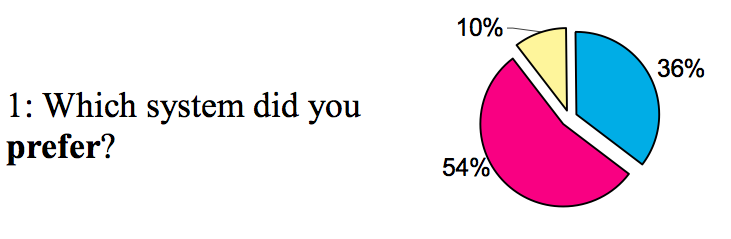
\includegraphics[width=0.6\textwidth]{figures-bharath/firstQ_liveUser.png}
%  \caption{Final Questionnaire - Question 1 \\(Blue - Apriori, Pink - MAUT, Yellow - No difference)(\cite{liveUserStudy}}
%\label{fig:q1}
%    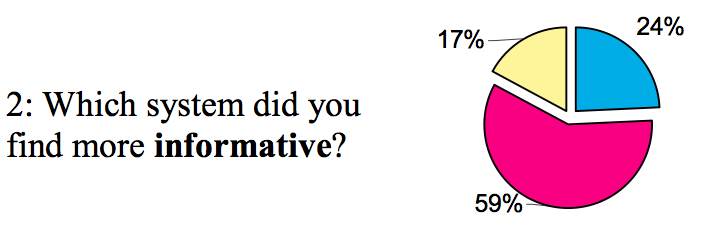
\includegraphics[width=0.6\textwidth]{figures-bharath/secondQ_liveUser.png}
%  \caption{Final Questionnaire - Question 2 (\cite{liveUserStudy}}
%\label{fig:q2}
%\end{figure}
\textbf{Recommendation Efficiency:} To be successful, recommender systems must be able to quickly and efficiently guide a user through a product-space. 
Shorter the length of recommendation session, better is the recommendation efficiency.
Sequencing bias was eliminated by randomizing the presentation order in terms of critiquing technique and dataset.
The average session length for two trials for both camera and PC datasets is shown in Table \ref{tab:liveUserStudies}.
For the camera dataset, MAUT performed better (3.8 cycles) compared to Apriori (7.3 cycles).
But for the PC dataset, Apriori performed better (6.4 cycles) compared to MAUT (8.5 cycles).
A possible explanation as to why Apriori performed better in PC domain and MAUT performed better in camera domain is that Apriori is likely to perform on larger and more complex datasets.
Overall, both recommenders are quite efficient.\\
\\
\textbf{Recommendation Accuracy:} 
Recommenders should also be measured by the \textit{quality} or \textit{accuracy} of the recommendations made to users over the course of a session. 
After a user has interacted with the recommender system and chosen a product $p$, he is asked to view the entire catalog of products. 
The user is then asked whether he is willing to retain $p$  or change it for another better product in the catalog.
The accuracy of the recommender is evaluated in terms of percentage of times that the user chooses to retain his selected product($p$).
Higher the number of times a user retains the selected product($p$), higher is the accuracy of the recommender system.
Accuracy results for both approaches are shown in Table \ref{tab:liveUserStudies}.
MAUT achieves 68.4\% accuracy on PC dataset and 82.5\% accuracy on camera dataset.
Apriori achieves 57.9\% and 64.6\% accuracy on PC and camera datasets respectively.
Therefore, MAUT seems to be recommending optimal products to the users. \\
\\
\textbf{User Experience:}
After users have interacted with both the recommender systems, they were asked to fill out a questionnaire in order to gauge their level of satisfaction with the system.
Some of the questions were: "I found the compound critiques easy to understand", "The compound critiques were relevant to my preferences", "I would use this recommender in the future to buy other products" etc.
Users were asked to give a score of -2 to +2 for each of these statements, where -2 is strongly disagree and +2 is strongly agree.
Both systems received a positive feedback from the questionnaires, but most results were strongly in favor of MAUT-based approach.
The final questionnaire simply asked the user to vote which system (Apriori or MAUT) performed better in terms of various criteria such as overall performance, informativeness etc. 

The conclusion of this study is that the Apriori-based approach has an advantage when it comes to producing more efficient sessions in complex product spaces but the MAUT-based approach tends to produce higher quality recommendations. 

